\documentclass[aspectratio=169]{beamer}

\usetheme{Boadilla}
\usefonttheme{professionalfonts}
\setbeamertemplate{navigation symbols}{}
\setbeamertemplate{itemize items}[circle]
\setbeamertemplate{enumerate items}[default]
\setbeamertemplate{headline}{}

\usepackage[utf8]{inputenc}
\usepackage[T1]{fontenc}
\usepackage{lmodern}
\usepackage{amsmath}
\usepackage{booktabs}
\usepackage{tabularx}
\usepackage{array}
\usepackage{hyperref}
\usepackage[strings]{underscore}
\usepackage{listings}
\usepackage{tikz}
\usetikzlibrary{arrows.meta,positioning,fit,calc,shapes.geometric}
\usepackage{xcolor}

\definecolor{courseblue}{HTML}{12355B}
\definecolor{coursegold}{HTML}{C98A2E}
\definecolor{courseice}{HTML}{EEF3F8}
\definecolor{coursegreen}{HTML}{2F6B4F}
\definecolor{coursegray}{HTML}{4B5563}
\definecolor{codebg}{HTML}{F7F9FC}
\definecolor{codecomment}{HTML}{5E6C84}
\definecolor{codestring}{HTML}{0B6E4F}

\setbeamercolor{palette primary}{bg=courseblue,fg=white}
\setbeamercolor{palette secondary}{bg=coursegold,fg=white}
\setbeamercolor{palette tertiary}{bg=courseblue,fg=white}
\setbeamercolor{palette quaternary}{bg=coursegold,fg=white}
\setbeamercolor{structure}{fg=courseblue}
\setbeamercolor{frametitle}{bg=courseice,fg=courseblue}
\setbeamercolor{title}{fg=courseblue}
\setbeamercolor{block title}{bg=courseblue,fg=white}
\setbeamercolor{block body}{bg=courseice,fg=black}
\setbeamercolor{normal text}{fg=black,bg=white}
\setbeamercolor{alerted text}{fg=coursegold}

\setbeamerfont{footline}{size=\scriptsize}

\setbeamertemplate{footline}{
  \leavevmode
  \hbox{
    \begin{beamercolorbox}[wd=.33\paperwidth,ht=2.8ex,dp=1.2ex,leftskip=0.8em]{palette primary}%
      University of Trieste
    \end{beamercolorbox}%
    \begin{beamercolorbox}[wd=.49\paperwidth,ht=2.8ex,dp=1.2ex,center]{palette tertiary}%
      \coursename{} \textbar{} \coursecode
    \end{beamercolorbox}%
    \begin{beamercolorbox}[wd=.18\paperwidth,ht=2.8ex,dp=1.2ex,rightskip=0.8em plus1fil]{palette secondary}%
      \insertframenumber{} / \inserttotalframenumber
    \end{beamercolorbox}%
  }
}

\hypersetup{
  colorlinks=true,
  linkcolor=courseblue,
  urlcolor=coursegreen
}

\lstdefinestyle{coursepython}{
  language=Python,
  basicstyle=\ttfamily\footnotesize,
  keywordstyle=\color{courseblue}\bfseries,
  commentstyle=\color{codecomment}\itshape,
  stringstyle=\color{codestring},
  showstringspaces=false,
  columns=fullflexible,
  keepspaces=true,
  frame=single,
  framerule=0.6pt,
  rulecolor=\color{courseblue},
  backgroundcolor=\color{codebg},
  xleftmargin=0.4em,
  xrightmargin=0.4em,
  aboveskip=0.4em,
  belowskip=0.2em
}

\newcommand{\coursename}{Data-driven Systems Engineering}
\newcommand{\coursecode}{440MI / 305SM}
\newcommand{\coursefooter}{}

\newcommand{\learninggoals}[1]{
  \begin{block}{Learning goals}
  #1
  \end{block}
}

\newcommand{\repoactivity}[1]{
  \begin{block}{Repo activity}
  #1
  \end{block}
}

\newcommand{\readinglist}[1]{
  \begin{block}{Papers and materials}
  {\footnotesize #1}
  \end{block}
}

\newcommand{\coursecontextframe}[5]{
  \begin{frame}{Course Map and Running Cases}
  \centering
  \begin{tikzpicture}[node distance=0.28cm]
  \node[flowbox, minimum width=1.45cm, minimum height=0.8cm] (problem) {\scriptsize Problem};
  \node[flowbox, minimum width=1.45cm, minimum height=0.8cm, right=of problem] (data) {\scriptsize Data};
  \node[flowbox, minimum width=1.45cm, minimum height=0.8cm, right=of data] (features) {\scriptsize Features};
  \node[flowbox, minimum width=1.45cm, minimum height=0.8cm, right=of features] (model) {\scriptsize Model};
  \node[flowbox, minimum width=1.45cm, minimum height=0.8cm, right=of model] (interface) {\scriptsize Interface};
  \node[flowbox, minimum width=1.45cm, minimum height=0.8cm, right=of interface] (delivery) {\scriptsize Delivery};
  \node[flowbox, minimum width=1.45cm, minimum height=0.8cm, right=of delivery] (monitor) {\scriptsize Monitor};
  \node[accentbox, minimum width=1.6cm, minimum height=0.8cm, right=of monitor] (evolution) {\scriptsize Evolution};
  \foreach \a/\b in {problem/data,data/features,features/model,model/interface,interface/delivery,delivery/monitor,monitor/evolution} {
    \draw[arrow] (\a) -- (\b);
  }
  \end{tikzpicture}

  \vspace{0.5em}
  \begin{block}{Today in the course}
  \textbf{Focus:} #1

  \textbf{Bridge:} #2
  \end{block}

  \begin{columns}[T]
  \column{0.48\textwidth}
  \begin{block}{Fraud case}
  {\footnotesize #3}
  \end{block}
  \column{0.48\textwidth}
  \begin{block}{Pasteurization case}
  {\footnotesize #4}
  \end{block}
  \end{columns}

  \vspace{0.3em}
  {\footnotesize \textbf{Course thread:} #5}
  \coursefooter
  \end{frame}
}

\newcommand{\classclosingframe}[4]{
  \begin{frame}{From This Class to the Next}
  \begin{block}{What stays with us}
  #1
  \end{block}

  \begin{columns}[T]
  \column{0.48\textwidth}
  \begin{block}{Project use}
  {\footnotesize #2}
  \end{block}
  \column{0.48\textwidth}
  \begin{block}{Next connection}
  {\footnotesize #3}
  \end{block}
  \end{columns}

  \vspace{0.3em}
  {\footnotesize \textbf{Course thread:} #4}
  \coursefooter
  \end{frame}
}

\tikzset{
  flowbox/.style={
    rounded corners=3pt,
    draw=courseblue,
    fill=courseice,
    very thick,
    minimum width=2.2cm,
    minimum height=0.9cm,
    align=center,
    font=\small
  },
  accentbox/.style={
    rounded corners=3pt,
    draw=coursegold,
    fill=coursegold!15,
    very thick,
    minimum width=2.2cm,
    minimum height=0.9cm,
    align=center,
    font=\small
  },
  arrow/.style={
    -{Latex[length=2.5mm,width=2mm]},
    thick,
    draw=courseblue
  }
}

% Visual layer on top of common.tex: tiles, icons, a progress-strip section divider, and a footer
% strip that defines the concepts appearing for the first time on each slide.
% Same look as the Class 20 deck. Load with:  \documentclass[aspectratio=169]{beamer}

\usetheme{Boadilla}
\usefonttheme{professionalfonts}
\setbeamertemplate{navigation symbols}{}
\setbeamertemplate{itemize items}[circle]
\setbeamertemplate{enumerate items}[default]
\setbeamertemplate{headline}{}

\usepackage[utf8]{inputenc}
\usepackage[T1]{fontenc}
\usepackage{lmodern}
\usepackage{amsmath}
\usepackage{booktabs}
\usepackage{tabularx}
\usepackage{array}
\usepackage{hyperref}
\usepackage[strings]{underscore}
\usepackage{listings}
\usepackage{tikz}
\usetikzlibrary{arrows.meta,positioning,fit,calc,shapes.geometric}
\usepackage{xcolor}

\definecolor{courseblue}{HTML}{12355B}
\definecolor{coursegold}{HTML}{C98A2E}
\definecolor{courseice}{HTML}{EEF3F8}
\definecolor{coursegreen}{HTML}{2F6B4F}
\definecolor{coursegray}{HTML}{4B5563}
\definecolor{codebg}{HTML}{F7F9FC}
\definecolor{codecomment}{HTML}{5E6C84}
\definecolor{codestring}{HTML}{0B6E4F}

\setbeamercolor{palette primary}{bg=courseblue,fg=white}
\setbeamercolor{palette secondary}{bg=coursegold,fg=white}
\setbeamercolor{palette tertiary}{bg=courseblue,fg=white}
\setbeamercolor{palette quaternary}{bg=coursegold,fg=white}
\setbeamercolor{structure}{fg=courseblue}
\setbeamercolor{frametitle}{bg=courseice,fg=courseblue}
\setbeamercolor{title}{fg=courseblue}
\setbeamercolor{block title}{bg=courseblue,fg=white}
\setbeamercolor{block body}{bg=courseice,fg=black}
\setbeamercolor{normal text}{fg=black,bg=white}
\setbeamercolor{alerted text}{fg=coursegold}

\setbeamerfont{footline}{size=\scriptsize}

\setbeamertemplate{footline}{
  \leavevmode
  \hbox{
    \begin{beamercolorbox}[wd=.33\paperwidth,ht=2.8ex,dp=1.2ex,leftskip=0.8em]{palette primary}%
      University of Trieste
    \end{beamercolorbox}%
    \begin{beamercolorbox}[wd=.49\paperwidth,ht=2.8ex,dp=1.2ex,center]{palette tertiary}%
      \coursename{} \textbar{} \coursecode
    \end{beamercolorbox}%
    \begin{beamercolorbox}[wd=.18\paperwidth,ht=2.8ex,dp=1.2ex,rightskip=0.8em plus1fil]{palette secondary}%
      \insertframenumber{} / \inserttotalframenumber
    \end{beamercolorbox}%
  }
}

\hypersetup{
  colorlinks=true,
  linkcolor=courseblue,
  urlcolor=coursegreen
}

\lstdefinestyle{coursepython}{
  language=Python,
  basicstyle=\ttfamily\footnotesize,
  keywordstyle=\color{courseblue}\bfseries,
  commentstyle=\color{codecomment}\itshape,
  stringstyle=\color{codestring},
  showstringspaces=false,
  columns=fullflexible,
  keepspaces=true,
  frame=single,
  framerule=0.6pt,
  rulecolor=\color{courseblue},
  backgroundcolor=\color{codebg},
  xleftmargin=0.4em,
  xrightmargin=0.4em,
  aboveskip=0.4em,
  belowskip=0.2em
}

\newcommand{\coursename}{Data-driven Systems Engineering}
\newcommand{\coursecode}{440MI / 305SM}
\newcommand{\coursefooter}{}

\newcommand{\learninggoals}[1]{
  \begin{block}{Learning goals}
  #1
  \end{block}
}

\newcommand{\repoactivity}[1]{
  \begin{block}{Repo activity}
  #1
  \end{block}
}

\newcommand{\readinglist}[1]{
  \begin{block}{Papers and materials}
  {\footnotesize #1}
  \end{block}
}

\newcommand{\coursecontextframe}[5]{
  \begin{frame}{Course Map and Running Cases}
  \centering
  \begin{tikzpicture}[node distance=0.28cm]
  \node[flowbox, minimum width=1.45cm, minimum height=0.8cm] (problem) {\scriptsize Problem};
  \node[flowbox, minimum width=1.45cm, minimum height=0.8cm, right=of problem] (data) {\scriptsize Data};
  \node[flowbox, minimum width=1.45cm, minimum height=0.8cm, right=of data] (features) {\scriptsize Features};
  \node[flowbox, minimum width=1.45cm, minimum height=0.8cm, right=of features] (model) {\scriptsize Model};
  \node[flowbox, minimum width=1.45cm, minimum height=0.8cm, right=of model] (interface) {\scriptsize Interface};
  \node[flowbox, minimum width=1.45cm, minimum height=0.8cm, right=of interface] (delivery) {\scriptsize Delivery};
  \node[flowbox, minimum width=1.45cm, minimum height=0.8cm, right=of delivery] (monitor) {\scriptsize Monitor};
  \node[accentbox, minimum width=1.6cm, minimum height=0.8cm, right=of monitor] (evolution) {\scriptsize Evolution};
  \foreach \a/\b in {problem/data,data/features,features/model,model/interface,interface/delivery,delivery/monitor,monitor/evolution} {
    \draw[arrow] (\a) -- (\b);
  }
  \end{tikzpicture}

  \vspace{0.5em}
  \begin{block}{Today in the course}
  \textbf{Focus:} #1

  \textbf{Bridge:} #2
  \end{block}

  \begin{columns}[T]
  \column{0.48\textwidth}
  \begin{block}{Fraud case}
  {\footnotesize #3}
  \end{block}
  \column{0.48\textwidth}
  \begin{block}{Pasteurization case}
  {\footnotesize #4}
  \end{block}
  \end{columns}

  \vspace{0.3em}
  {\footnotesize \textbf{Course thread:} #5}
  \coursefooter
  \end{frame}
}

\newcommand{\classclosingframe}[4]{
  \begin{frame}{From This Class to the Next}
  \begin{block}{What stays with us}
  #1
  \end{block}

  \begin{columns}[T]
  \column{0.48\textwidth}
  \begin{block}{Project use}
  {\footnotesize #2}
  \end{block}
  \column{0.48\textwidth}
  \begin{block}{Next connection}
  {\footnotesize #3}
  \end{block}
  \end{columns}

  \vspace{0.3em}
  {\footnotesize \textbf{Course thread:} #4}
  \coursefooter
  \end{frame}
}

\tikzset{
  flowbox/.style={
    rounded corners=3pt,
    draw=courseblue,
    fill=courseice,
    very thick,
    minimum width=2.2cm,
    minimum height=0.9cm,
    align=center,
    font=\small
  },
  accentbox/.style={
    rounded corners=3pt,
    draw=coursegold,
    fill=coursegold!15,
    very thick,
    minimum width=2.2cm,
    minimum height=0.9cm,
    align=center,
    font=\small
  },
  arrow/.style={
    -{Latex[length=2.5mm,width=2mm]},
    thick,
    draw=courseblue
  }
}
  % Visual layer on top of common.tex: tiles, icons, a progress-strip section divider, and a footer
% strip that defines the concepts appearing for the first time on each slide.
% Same look as the Class 20 deck. Load with:  \documentclass[aspectratio=169]{beamer}

\usetheme{Boadilla}
\usefonttheme{professionalfonts}
\setbeamertemplate{navigation symbols}{}
\setbeamertemplate{itemize items}[circle]
\setbeamertemplate{enumerate items}[default]
\setbeamertemplate{headline}{}

\usepackage[utf8]{inputenc}
\usepackage[T1]{fontenc}
\usepackage{lmodern}
\usepackage{amsmath}
\usepackage{booktabs}
\usepackage{tabularx}
\usepackage{array}
\usepackage{hyperref}
\usepackage[strings]{underscore}
\usepackage{listings}
\usepackage{tikz}
\usetikzlibrary{arrows.meta,positioning,fit,calc,shapes.geometric}
\usepackage{xcolor}

\definecolor{courseblue}{HTML}{12355B}
\definecolor{coursegold}{HTML}{C98A2E}
\definecolor{courseice}{HTML}{EEF3F8}
\definecolor{coursegreen}{HTML}{2F6B4F}
\definecolor{coursegray}{HTML}{4B5563}
\definecolor{codebg}{HTML}{F7F9FC}
\definecolor{codecomment}{HTML}{5E6C84}
\definecolor{codestring}{HTML}{0B6E4F}

\setbeamercolor{palette primary}{bg=courseblue,fg=white}
\setbeamercolor{palette secondary}{bg=coursegold,fg=white}
\setbeamercolor{palette tertiary}{bg=courseblue,fg=white}
\setbeamercolor{palette quaternary}{bg=coursegold,fg=white}
\setbeamercolor{structure}{fg=courseblue}
\setbeamercolor{frametitle}{bg=courseice,fg=courseblue}
\setbeamercolor{title}{fg=courseblue}
\setbeamercolor{block title}{bg=courseblue,fg=white}
\setbeamercolor{block body}{bg=courseice,fg=black}
\setbeamercolor{normal text}{fg=black,bg=white}
\setbeamercolor{alerted text}{fg=coursegold}

\setbeamerfont{footline}{size=\scriptsize}

\setbeamertemplate{footline}{
  \leavevmode
  \hbox{
    \begin{beamercolorbox}[wd=.33\paperwidth,ht=2.8ex,dp=1.2ex,leftskip=0.8em]{palette primary}%
      University of Trieste
    \end{beamercolorbox}%
    \begin{beamercolorbox}[wd=.49\paperwidth,ht=2.8ex,dp=1.2ex,center]{palette tertiary}%
      \coursename{} \textbar{} \coursecode
    \end{beamercolorbox}%
    \begin{beamercolorbox}[wd=.18\paperwidth,ht=2.8ex,dp=1.2ex,rightskip=0.8em plus1fil]{palette secondary}%
      \insertframenumber{} / \inserttotalframenumber
    \end{beamercolorbox}%
  }
}

\hypersetup{
  colorlinks=true,
  linkcolor=courseblue,
  urlcolor=coursegreen
}

\lstdefinestyle{coursepython}{
  language=Python,
  basicstyle=\ttfamily\footnotesize,
  keywordstyle=\color{courseblue}\bfseries,
  commentstyle=\color{codecomment}\itshape,
  stringstyle=\color{codestring},
  showstringspaces=false,
  columns=fullflexible,
  keepspaces=true,
  frame=single,
  framerule=0.6pt,
  rulecolor=\color{courseblue},
  backgroundcolor=\color{codebg},
  xleftmargin=0.4em,
  xrightmargin=0.4em,
  aboveskip=0.4em,
  belowskip=0.2em
}

\newcommand{\coursename}{Data-driven Systems Engineering}
\newcommand{\coursecode}{440MI / 305SM}
\newcommand{\coursefooter}{}

\newcommand{\learninggoals}[1]{
  \begin{block}{Learning goals}
  #1
  \end{block}
}

\newcommand{\repoactivity}[1]{
  \begin{block}{Repo activity}
  #1
  \end{block}
}

\newcommand{\readinglist}[1]{
  \begin{block}{Papers and materials}
  {\footnotesize #1}
  \end{block}
}

\newcommand{\coursecontextframe}[5]{
  \begin{frame}{Course Map and Running Cases}
  \centering
  \begin{tikzpicture}[node distance=0.28cm]
  \node[flowbox, minimum width=1.45cm, minimum height=0.8cm] (problem) {\scriptsize Problem};
  \node[flowbox, minimum width=1.45cm, minimum height=0.8cm, right=of problem] (data) {\scriptsize Data};
  \node[flowbox, minimum width=1.45cm, minimum height=0.8cm, right=of data] (features) {\scriptsize Features};
  \node[flowbox, minimum width=1.45cm, minimum height=0.8cm, right=of features] (model) {\scriptsize Model};
  \node[flowbox, minimum width=1.45cm, minimum height=0.8cm, right=of model] (interface) {\scriptsize Interface};
  \node[flowbox, minimum width=1.45cm, minimum height=0.8cm, right=of interface] (delivery) {\scriptsize Delivery};
  \node[flowbox, minimum width=1.45cm, minimum height=0.8cm, right=of delivery] (monitor) {\scriptsize Monitor};
  \node[accentbox, minimum width=1.6cm, minimum height=0.8cm, right=of monitor] (evolution) {\scriptsize Evolution};
  \foreach \a/\b in {problem/data,data/features,features/model,model/interface,interface/delivery,delivery/monitor,monitor/evolution} {
    \draw[arrow] (\a) -- (\b);
  }
  \end{tikzpicture}

  \vspace{0.5em}
  \begin{block}{Today in the course}
  \textbf{Focus:} #1

  \textbf{Bridge:} #2
  \end{block}

  \begin{columns}[T]
  \column{0.48\textwidth}
  \begin{block}{Fraud case}
  {\footnotesize #3}
  \end{block}
  \column{0.48\textwidth}
  \begin{block}{Pasteurization case}
  {\footnotesize #4}
  \end{block}
  \end{columns}

  \vspace{0.3em}
  {\footnotesize \textbf{Course thread:} #5}
  \coursefooter
  \end{frame}
}

\newcommand{\classclosingframe}[4]{
  \begin{frame}{From This Class to the Next}
  \begin{block}{What stays with us}
  #1
  \end{block}

  \begin{columns}[T]
  \column{0.48\textwidth}
  \begin{block}{Project use}
  {\footnotesize #2}
  \end{block}
  \column{0.48\textwidth}
  \begin{block}{Next connection}
  {\footnotesize #3}
  \end{block}
  \end{columns}

  \vspace{0.3em}
  {\footnotesize \textbf{Course thread:} #4}
  \coursefooter
  \end{frame}
}

\tikzset{
  flowbox/.style={
    rounded corners=3pt,
    draw=courseblue,
    fill=courseice,
    very thick,
    minimum width=2.2cm,
    minimum height=0.9cm,
    align=center,
    font=\small
  },
  accentbox/.style={
    rounded corners=3pt,
    draw=coursegold,
    fill=coursegold!15,
    very thick,
    minimum width=2.2cm,
    minimum height=0.9cm,
    align=center,
    font=\small
  },
  arrow/.style={
    -{Latex[length=2.5mm,width=2mm]},
    thick,
    draw=courseblue
  }
}
  % Visual layer on top of common.tex: tiles, icons, a progress-strip section divider, and a footer
% strip that defines the concepts appearing for the first time on each slide.
% Same look as the Class 20 deck. Load with:  \input{common}  \input{common_visual}
%
% Before the first \sectiondivider, a deck must define
%   \sectioncount   the number of sections, e.g. 4
%   \sectionlabels  a \foreach list of number/label pairs, e.g. 1/Need,2/Testable,3/Manage,4/Practice
% Icons come from the fontawesome5 package (Font Awesome 5 Free), e.g. \faIcon{robot}.

\usepackage{colortbl}
\usepackage{fontawesome5}
\usetikzlibrary{backgrounds}

% Slides read better without automatic hyphenation.
\hyphenpenalty=10000
\exhyphenpenalty=10000

\definecolor{coursered}{HTML}{A23B2A}
\newcommand{\goldink}{\color{coursegold!65!black}}

\tikzset{
  tile/.style={rounded corners=4pt, fill=courseice, draw=none, align=center, font=\footnotesize, inner sep=5pt},
  tileblue/.style={tile, fill=white, draw=courseblue!55, thick},
  tilegold/.style={tile, fill=coursegold!14, draw=coursegold, thick},
  tilegreen/.style={tile, fill=coursegreen!10, draw=coursegreen!70, thick},
  tilered/.style={tile, fill=coursered!8, draw=coursered!70, thick},
  tilegray/.style={tile, fill=white, draw=coursegray!55, thick, dashed},
  tag/.style={rounded corners=2pt, fill=coursegold, text=white, font=\bfseries\tiny, inner sep=2.5pt},
  chip/.style={rounded corners=3pt, fill=courseblue, text=white, font=\footnotesize\bfseries, align=center, inner sep=4pt},
  note/.style={font=\scriptsize, text=coursegray, align=left},
  arrowgold/.style={-{Latex[length=2.5mm,width=2mm]}, thick, draw=coursegold},
  arrowred/.style={-{Latex[length=2.5mm,width=2mm]}, thick, draw=coursered},
  arrowgreen/.style={-{Latex[length=2.5mm,width=2mm]}, thick, draw=coursegreen},
  arrowgray/.style={-{Latex[length=2mm,width=1.6mm]}, thick, draw=coursegray!70},
}

% A round icon badge, drawn inside a tikzpicture: x y colour icon
\newcommand{\badge}[4]{%
  \node[circle, fill=#3, text=white, minimum size=0.85cm, inner sep=0pt] at (#1,#2) {\large\faIcon{#4}};
}

% Inline tags for the kind of requirement.
\newcommand{\Ftag}{\colorbox{courseblue}{\color{white}\bfseries\scriptsize\ \ F\ \ }}
\newcommand{\NFtag}{\colorbox{coursegold}{\color{white}\bfseries\scriptsize\ NF\ }}
\newcommand{\Dtag}{\colorbox{coursegreen}{\color{white}\bfseries\scriptsize\ \ D\ \ }}
\newcommand{\MLtag}{\colorbox{coursered}{\color{white}\bfseries\scriptsize\ ML\ }}

% Footer: a strip with the concepts that appear for the first time on the slide, above the
% usual bar. The bar total counts only the main lecture; a backup slide is numbered separately.
\makeatletter
\def\conceptstext{}
\def\currentsectionname{}
\setbeamercolor{conceptbar}{bg=coursegold!12,fg=black}
\newcommand{\cterm}[2]{{\bfseries\color{courseblue}#1:}\ #2\hspace{0.8em}}
\newcommand{\newtag}{\colorbox{coursegold}{\color{white}\bfseries\tiny\ NEW\ }\hspace{0.6em}}
\setbeamertemplate{footline}{
  \leavevmode
  \vbox{%
    \ifx\conceptstext\empty\else
      \hbox{\color{coursegold}\rule{\paperwidth}{0.8pt}}%
      \hbox{\begin{beamercolorbox}[wd=\paperwidth,leftskip=0.5cm,rightskip=0.5cm,sep=3pt]{conceptbar}\scriptsize\newtag\conceptstext\end{beamercolorbox}}%
    \fi
    \hbox{%
      \begin{beamercolorbox}[wd=.33\paperwidth,ht=2.8ex,dp=1.2ex,leftskip=0.8em]{palette primary}%
        \ifbeamer@inappendix Backup\else\ifnum\value{section}>0 \arabic{section}\ \textbar\ \currentsectionname\else University of Trieste\fi\fi
      \end{beamercolorbox}%
      \begin{beamercolorbox}[wd=.49\paperwidth,ht=2.8ex,dp=1.2ex,center]{palette tertiary}%
        \coursename{} \textbar{} \coursecode
      \end{beamercolorbox}%
      \begin{beamercolorbox}[wd=.18\paperwidth,ht=2.8ex,dp=1.2ex,right,rightskip=0.8em]{palette secondary}%
        \ifbeamer@inappendix Backup \insertframenumberinappendix\else\insertframenumber{} / \insertmainframenumber\fi
      \end{beamercolorbox}%
    }}}
\makeatother
\newenvironment{cframe}[2]{\gdef\conceptstext{#2}\begin{frame}{#1}}{\end{frame}\gdef\conceptstext{}}

% Section divider: progress strip, recap of the previous part, and the roadmap of the next one.
% Arguments: number, title, icon, previously, items.
\newcommand{\sectiondivider}[5]{%
  \section{#2}\gdef\currentsectionname{#2}
  \begin{frame}
  \centering
  \begin{tikzpicture}
  \pgfmathsetmacro{\chipw}{13.6/\sectioncount}
  \foreach \i/\lab in \sectionlabels {
    \ifnum\i<#1 \def\chipfill{courseblue!22}\def\chiptext{courseblue}\else
    \ifnum\i=#1 \def\chipfill{courseblue}\def\chiptext{white}\else
    \def\chipfill{courseice}\def\chiptext{coursegray}\fi\fi
    \node[rounded corners=3pt, minimum width={(\chipw-0.1)*1cm}, minimum height=0.6cm, font=\scriptsize\bfseries, fill=\chipfill, text=\chiptext] at ({\chipw/2+(\i-1)*\chipw},0) {\i\ \lab};
  }
  \node[circle, fill=courseblue, text=white, font=\Huge\bfseries, minimum size=1.7cm, inner sep=0] at (1.0,-1.7) {#1};
  \node[anchor=west, font=\huge\bfseries, text=courseblue, text width=8.8cm, align=left] at (2.2,-1.7) {#2};
  \node[circle, fill=coursegold!16, draw=coursegold, thick, text=coursegold!75!black, font=\fontsize{26}{26}\selectfont, minimum size=1.9cm, inner sep=0] at (12.6,-1.7) {\faIcon{#3}};
  \ifx\relax#4\relax\else
    \node[anchor=north west, font=\small\itshape, text=coursegray, text width=13.2cm, align=left] at (0.1,-2.95) {Previously: #4};
  \fi
  \node[anchor=north west, font=\footnotesize\bfseries, text=coursegold!65!black] at (0.1,-3.95) {IN THIS PART};
  \node[anchor=north west, font=\small, text width=13.2cm, align=left] at (0.1,-4.35) {#5};
  \end{tikzpicture}
  \end{frame}
}

%
% Before the first \sectiondivider, a deck must define
%   \sectioncount   the number of sections, e.g. 4
%   \sectionlabels  a \foreach list of number/label pairs, e.g. 1/Need,2/Testable,3/Manage,4/Practice
% Icons come from the fontawesome5 package (Font Awesome 5 Free), e.g. \faIcon{robot}.

\usepackage{colortbl}
\usepackage{fontawesome5}
\usetikzlibrary{backgrounds}

% Slides read better without automatic hyphenation.
\hyphenpenalty=10000
\exhyphenpenalty=10000

\definecolor{coursered}{HTML}{A23B2A}
\newcommand{\goldink}{\color{coursegold!65!black}}

\tikzset{
  tile/.style={rounded corners=4pt, fill=courseice, draw=none, align=center, font=\footnotesize, inner sep=5pt},
  tileblue/.style={tile, fill=white, draw=courseblue!55, thick},
  tilegold/.style={tile, fill=coursegold!14, draw=coursegold, thick},
  tilegreen/.style={tile, fill=coursegreen!10, draw=coursegreen!70, thick},
  tilered/.style={tile, fill=coursered!8, draw=coursered!70, thick},
  tilegray/.style={tile, fill=white, draw=coursegray!55, thick, dashed},
  tag/.style={rounded corners=2pt, fill=coursegold, text=white, font=\bfseries\tiny, inner sep=2.5pt},
  chip/.style={rounded corners=3pt, fill=courseblue, text=white, font=\footnotesize\bfseries, align=center, inner sep=4pt},
  note/.style={font=\scriptsize, text=coursegray, align=left},
  arrowgold/.style={-{Latex[length=2.5mm,width=2mm]}, thick, draw=coursegold},
  arrowred/.style={-{Latex[length=2.5mm,width=2mm]}, thick, draw=coursered},
  arrowgreen/.style={-{Latex[length=2.5mm,width=2mm]}, thick, draw=coursegreen},
  arrowgray/.style={-{Latex[length=2mm,width=1.6mm]}, thick, draw=coursegray!70},
}

% A round icon badge, drawn inside a tikzpicture: x y colour icon
\newcommand{\badge}[4]{%
  \node[circle, fill=#3, text=white, minimum size=0.85cm, inner sep=0pt] at (#1,#2) {\large\faIcon{#4}};
}

% Inline tags for the kind of requirement.
\newcommand{\Ftag}{\colorbox{courseblue}{\color{white}\bfseries\scriptsize\ \ F\ \ }}
\newcommand{\NFtag}{\colorbox{coursegold}{\color{white}\bfseries\scriptsize\ NF\ }}
\newcommand{\Dtag}{\colorbox{coursegreen}{\color{white}\bfseries\scriptsize\ \ D\ \ }}
\newcommand{\MLtag}{\colorbox{coursered}{\color{white}\bfseries\scriptsize\ ML\ }}

% Footer: a strip with the concepts that appear for the first time on the slide, above the
% usual bar. The bar total counts only the main lecture; a backup slide is numbered separately.
\makeatletter
\def\conceptstext{}
\def\currentsectionname{}
\setbeamercolor{conceptbar}{bg=coursegold!12,fg=black}
\newcommand{\cterm}[2]{{\bfseries\color{courseblue}#1:}\ #2\hspace{0.8em}}
\newcommand{\newtag}{\colorbox{coursegold}{\color{white}\bfseries\tiny\ NEW\ }\hspace{0.6em}}
\setbeamertemplate{footline}{
  \leavevmode
  \vbox{%
    \ifx\conceptstext\empty\else
      \hbox{\color{coursegold}\rule{\paperwidth}{0.8pt}}%
      \hbox{\begin{beamercolorbox}[wd=\paperwidth,leftskip=0.5cm,rightskip=0.5cm,sep=3pt]{conceptbar}\scriptsize\newtag\conceptstext\end{beamercolorbox}}%
    \fi
    \hbox{%
      \begin{beamercolorbox}[wd=.33\paperwidth,ht=2.8ex,dp=1.2ex,leftskip=0.8em]{palette primary}%
        \ifbeamer@inappendix Backup\else\ifnum\value{section}>0 \arabic{section}\ \textbar\ \currentsectionname\else University of Trieste\fi\fi
      \end{beamercolorbox}%
      \begin{beamercolorbox}[wd=.49\paperwidth,ht=2.8ex,dp=1.2ex,center]{palette tertiary}%
        \coursename{} \textbar{} \coursecode
      \end{beamercolorbox}%
      \begin{beamercolorbox}[wd=.18\paperwidth,ht=2.8ex,dp=1.2ex,right,rightskip=0.8em]{palette secondary}%
        \ifbeamer@inappendix Backup \insertframenumberinappendix\else\insertframenumber{} / \insertmainframenumber\fi
      \end{beamercolorbox}%
    }}}
\makeatother
\newenvironment{cframe}[2]{\gdef\conceptstext{#2}\begin{frame}{#1}}{\end{frame}\gdef\conceptstext{}}

% Section divider: progress strip, recap of the previous part, and the roadmap of the next one.
% Arguments: number, title, icon, previously, items.
\newcommand{\sectiondivider}[5]{%
  \section{#2}\gdef\currentsectionname{#2}
  \begin{frame}
  \centering
  \begin{tikzpicture}
  \pgfmathsetmacro{\chipw}{13.6/\sectioncount}
  \foreach \i/\lab in \sectionlabels {
    \ifnum\i<#1 \def\chipfill{courseblue!22}\def\chiptext{courseblue}\else
    \ifnum\i=#1 \def\chipfill{courseblue}\def\chiptext{white}\else
    \def\chipfill{courseice}\def\chiptext{coursegray}\fi\fi
    \node[rounded corners=3pt, minimum width={(\chipw-0.1)*1cm}, minimum height=0.6cm, font=\scriptsize\bfseries, fill=\chipfill, text=\chiptext] at ({\chipw/2+(\i-1)*\chipw},0) {\i\ \lab};
  }
  \node[circle, fill=courseblue, text=white, font=\Huge\bfseries, minimum size=1.7cm, inner sep=0] at (1.0,-1.7) {#1};
  \node[anchor=west, font=\huge\bfseries, text=courseblue, text width=8.8cm, align=left] at (2.2,-1.7) {#2};
  \node[circle, fill=coursegold!16, draw=coursegold, thick, text=coursegold!75!black, font=\fontsize{26}{26}\selectfont, minimum size=1.9cm, inner sep=0] at (12.6,-1.7) {\faIcon{#3}};
  \ifx\relax#4\relax\else
    \node[anchor=north west, font=\small\itshape, text=coursegray, text width=13.2cm, align=left] at (0.1,-2.95) {Previously: #4};
  \fi
  \node[anchor=north west, font=\footnotesize\bfseries, text=coursegold!65!black] at (0.1,-3.95) {IN THIS PART};
  \node[anchor=north west, font=\small, text width=13.2cm, align=left] at (0.1,-4.35) {#5};
  \end{tikzpicture}
  \end{frame}
}

%
% Before the first \sectiondivider, a deck must define
%   \sectioncount   the number of sections, e.g. 4
%   \sectionlabels  a \foreach list of number/label pairs, e.g. 1/Need,2/Testable,3/Manage,4/Practice
% Icons come from the fontawesome5 package (Font Awesome 5 Free), e.g. \faIcon{robot}.

\usepackage{colortbl}
\usepackage{fontawesome5}
\usetikzlibrary{backgrounds}

% Slides read better without automatic hyphenation.
\hyphenpenalty=10000
\exhyphenpenalty=10000

\definecolor{coursered}{HTML}{A23B2A}
\newcommand{\goldink}{\color{coursegold!65!black}}

\tikzset{
  tile/.style={rounded corners=4pt, fill=courseice, draw=none, align=center, font=\footnotesize, inner sep=5pt},
  tileblue/.style={tile, fill=white, draw=courseblue!55, thick},
  tilegold/.style={tile, fill=coursegold!14, draw=coursegold, thick},
  tilegreen/.style={tile, fill=coursegreen!10, draw=coursegreen!70, thick},
  tilered/.style={tile, fill=coursered!8, draw=coursered!70, thick},
  tilegray/.style={tile, fill=white, draw=coursegray!55, thick, dashed},
  tag/.style={rounded corners=2pt, fill=coursegold, text=white, font=\bfseries\tiny, inner sep=2.5pt},
  chip/.style={rounded corners=3pt, fill=courseblue, text=white, font=\footnotesize\bfseries, align=center, inner sep=4pt},
  note/.style={font=\scriptsize, text=coursegray, align=left},
  arrowgold/.style={-{Latex[length=2.5mm,width=2mm]}, thick, draw=coursegold},
  arrowred/.style={-{Latex[length=2.5mm,width=2mm]}, thick, draw=coursered},
  arrowgreen/.style={-{Latex[length=2.5mm,width=2mm]}, thick, draw=coursegreen},
  arrowgray/.style={-{Latex[length=2mm,width=1.6mm]}, thick, draw=coursegray!70},
}

% A round icon badge, drawn inside a tikzpicture: x y colour icon
\newcommand{\badge}[4]{%
  \node[circle, fill=#3, text=white, minimum size=0.85cm, inner sep=0pt] at (#1,#2) {\large\faIcon{#4}};
}

% Inline tags for the kind of requirement.
\newcommand{\Ftag}{\colorbox{courseblue}{\color{white}\bfseries\scriptsize\ \ F\ \ }}
\newcommand{\NFtag}{\colorbox{coursegold}{\color{white}\bfseries\scriptsize\ NF\ }}
\newcommand{\Dtag}{\colorbox{coursegreen}{\color{white}\bfseries\scriptsize\ \ D\ \ }}
\newcommand{\MLtag}{\colorbox{coursered}{\color{white}\bfseries\scriptsize\ ML\ }}

% Footer: a strip with the concepts that appear for the first time on the slide, above the
% usual bar. The bar total counts only the main lecture; a backup slide is numbered separately.
\makeatletter
\def\conceptstext{}
\def\currentsectionname{}
\setbeamercolor{conceptbar}{bg=coursegold!12,fg=black}
\newcommand{\cterm}[2]{{\bfseries\color{courseblue}#1:}\ #2\hspace{0.8em}}
\newcommand{\newtag}{\colorbox{coursegold}{\color{white}\bfseries\tiny\ NEW\ }\hspace{0.6em}}
\setbeamertemplate{footline}{
  \leavevmode
  \vbox{%
    \ifx\conceptstext\empty\else
      \hbox{\color{coursegold}\rule{\paperwidth}{0.8pt}}%
      \hbox{\begin{beamercolorbox}[wd=\paperwidth,leftskip=0.5cm,rightskip=0.5cm,sep=3pt]{conceptbar}\scriptsize\newtag\conceptstext\end{beamercolorbox}}%
    \fi
    \hbox{%
      \begin{beamercolorbox}[wd=.33\paperwidth,ht=2.8ex,dp=1.2ex,leftskip=0.8em]{palette primary}%
        \ifbeamer@inappendix Backup\else\ifnum\value{section}>0 \arabic{section}\ \textbar\ \currentsectionname\else University of Trieste\fi\fi
      \end{beamercolorbox}%
      \begin{beamercolorbox}[wd=.49\paperwidth,ht=2.8ex,dp=1.2ex,center]{palette tertiary}%
        \coursename{} \textbar{} \coursecode
      \end{beamercolorbox}%
      \begin{beamercolorbox}[wd=.18\paperwidth,ht=2.8ex,dp=1.2ex,right,rightskip=0.8em]{palette secondary}%
        \ifbeamer@inappendix Backup \insertframenumberinappendix\else\insertframenumber{} / \insertmainframenumber\fi
      \end{beamercolorbox}%
    }}}
\makeatother
\newenvironment{cframe}[2]{\gdef\conceptstext{#2}\begin{frame}{#1}}{\end{frame}\gdef\conceptstext{}}

% Section divider: progress strip, recap of the previous part, and the roadmap of the next one.
% Arguments: number, title, icon, previously, items.
\newcommand{\sectiondivider}[5]{%
  \section{#2}\gdef\currentsectionname{#2}
  \begin{frame}
  \centering
  \begin{tikzpicture}
  \pgfmathsetmacro{\chipw}{13.6/\sectioncount}
  \foreach \i/\lab in \sectionlabels {
    \ifnum\i<#1 \def\chipfill{courseblue!22}\def\chiptext{courseblue}\else
    \ifnum\i=#1 \def\chipfill{courseblue}\def\chiptext{white}\else
    \def\chipfill{courseice}\def\chiptext{coursegray}\fi\fi
    \node[rounded corners=3pt, minimum width={(\chipw-0.1)*1cm}, minimum height=0.6cm, font=\scriptsize\bfseries, fill=\chipfill, text=\chiptext] at ({\chipw/2+(\i-1)*\chipw},0) {\i\ \lab};
  }
  \node[circle, fill=courseblue, text=white, font=\Huge\bfseries, minimum size=1.7cm, inner sep=0] at (1.0,-1.7) {#1};
  \node[anchor=west, font=\huge\bfseries, text=courseblue, text width=8.8cm, align=left] at (2.2,-1.7) {#2};
  \node[circle, fill=coursegold!16, draw=coursegold, thick, text=coursegold!75!black, font=\fontsize{26}{26}\selectfont, minimum size=1.9cm, inner sep=0] at (12.6,-1.7) {\faIcon{#3}};
  \ifx\relax#4\relax\else
    \node[anchor=north west, font=\small\itshape, text=coursegray, text width=13.2cm, align=left] at (0.1,-2.95) {Previously: #4};
  \fi
  \node[anchor=north west, font=\footnotesize\bfseries, text=coursegold!65!black] at (0.1,-3.95) {IN THIS PART};
  \node[anchor=north west, font=\small, text width=13.2cm, align=left] at (0.1,-4.35) {#5};
  \end{tikzpicture}
  \end{frame}
}


% Three parts; the progress strip on each divider uses these labels.
\newcommand{\sectioncount}{3}
\newcommand{\sectionlabels}{1/Process families,2/Agile foundations,3/Choosing for ML}

\title{Class 23: Process Models and Agile Foundations}
\author{\coursename}
\date{}

% ------------------------------------------------------------------ helpers
% A gold strip with the idea to remember: y text
\newcommand{\keyidea}[2]{%
  \node[tilegold, anchor=north west, minimum width=13.4cm, minimum height=0.8cm, text width=12.6cm, align=left, font=\footnotesize] at (0,#1) {{\bfseries\goldink\faIcon{lightbulb}\ Key idea.}\ #2};
}
% A goal card (6.6 x 1.5): x y style icon title text
\newcommand{\goalcard}[6]{%
  \node[#3, anchor=north west, minimum width=6.6cm, minimum height=1.7cm] at (#1,#2) {};
  \badge{#1+0.65}{#2-0.85}{courseblue}{#4}
  \node[anchor=west, text width=5.2cm, align=left, font=\small\bfseries, text=courseblue] at (#1+1.25,#2-0.3) {#5};
  \node[anchor=north west, text width=5.2cm, align=left, font=\footnotesize] at (#1+1.2,#2-0.55) {#6};
}
% One row of a three-column table: y icon label text gold-column text
\newcommand{\discchipw}{3.3}% width of the first column, in cm; a frame may change it locally
\newcommand{\discrow}[5]{%
  \node[chip, minimum width={\discchipw*1cm}, minimum height=0.68cm, font=\scriptsize\bfseries, anchor=west] at (0,#1) {\faIcon{#2}\ #3};
  \node[anchor=west, text width={(9.4-\discchipw-0.2)*1cm}, font=\scriptsize, align=left] at ({\discchipw+0.2},#1) {#4};
  \node[anchor=west, text width=3.9cm, font=\scriptsize\bfseries, align=left, text=courseblue] at (9.75,#1) {#5};
  \draw[courseice!70!courseblue, line width=0.5pt] (0,#1-0.42) -- (13.7,#1-0.42);
}
% One group of references: y height icon label text
\newcommand{\refrow}[5]{%
  \node[chip, anchor=west, minimum width=3.4cm, minimum height=0.68cm, font=\scriptsize\bfseries, align=left] at (0,#1-#2/2) {\faIcon{#3}\ #4};
  \node[anchor=west, text width=9.8cm, font=\scriptsize, align=left] at (3.6,#1-#2/2) {#5};
  \draw[courseice!70!courseblue, line width=0.5pt] (0,#1-#2) -- (13.7,#1-#2);
}
% A cell of the comparison grid: x y colour width text
\newcommand{\gridcell}[5]{%
  \node[tile, fill=white, draw=#3!55, thick, anchor=north west, minimum width=#4cm, minimum height=0.72cm, text width={(#4-0.3)*1cm}, align=left, font=\scriptsize] at (#1,#2) {#5};
}

\begin{document}

% ------------------------------------------------------------------ title
\frame{\titlepage \coursefooter}

% ------------------------------------------------------------------ goals
\begin{cframe}{Process models are decision tools}{\cterm{Process model}{a description of how software work is organized: activities, products, roles, and conditions.}\cterm{Hybrid process}{mixes plan-driven control with agile iteration.}}
\centering
\begin{tikzpicture}
\goalcard{0}{0}{tileblue}{balance-scale}{Compare}{Compare plan-driven, incremental, and hybrid approaches.}
\goalcard{6.8}{0}{tileblue}{code-branch}{Hybrid for ML}{Understand why ML projects often need hybrid processes.}
\goalcard{0}{-1.8}{tileblue}{sliders-h}{Match the context}{Match process choice to uncertainty, regulation, and team maturity.}
\goalcard{6.8}{-1.8}{tilegold}{shield-alt}{Trace the effects}{Explain how process decisions affect documentation, testing, and release risk.}
\node[tilegold, anchor=north west, minimum width=13.4cm, minimum height=0.85cm, text width=12.6cm, align=left, font=\footnotesize] at (0,-3.7) {{\bfseries\goldink\faIcon{link}\ Bridge from Class 22.} Requirements will change; the process decides how a team absorbs that change without losing control.};
\node[tilegold, fill=white, anchor=north west, minimum width=13.4cm, minimum height=0.8cm, text width=12.6cm, align=left, font=\footnotesize] at (0,-4.85) {{\color{courseblue}\faIcon{credit-card}}\ fraud scoring API \quad {\color{courseblue}\faIcon{thermometer-half}}\ pasteurization monitoring \quad {\color{courseblue}\faIcon{hospital}}\ hospital ML tool (contrast)};
\node[tag, anchor=west] at (0.25,-4.85) {RUNNING CASES};
\end{tikzpicture}
\coursefooter
\end{cframe}

% ------------------------------------------------------------------ roadmap
\begin{cframe}{Roadmap: three questions}{\cterm{Process family}{a group of processes that organize the same activities in a similar way.}}
\centering
\begin{tikzpicture}
\foreach \x/\n/\ico/\ttl/\q/\items in {0/1/sitemap/Process families/What does a process control?/{$\bullet$\ Plan-driven, incremental, agile\\[2pt]$\bullet$\ The same four activities, organized differently\\[2pt]$\bullet$\ The V-model}, 4.55/2/sync-alt/Agile foundations/{What did agile change, and what did it keep?}/{$\bullet$\ History and the manifesto\\[2pt]$\bullet$\ Principles adapted to ML teams\\[2pt]$\bullet$\ Definition of done and failure modes}, 9.1/3/compass/Choosing for ML/{Which process fits an ML system, and why?}/{$\bullet$\ Hybrid delivery and CRISP-DM\\[2pt]$\bullet$\ Gates between exploration and production\\[2pt]$\bullet$\ How to choose; a project checklist}} {
  \node[tile, anchor=north west, minimum width=4.3cm, minimum height=4.2cm] at (\x,0) {};
  \node[circle, fill=courseblue, text=white, font=\bfseries, minimum size=0.8cm, inner sep=0] at (\x+0.6,-0.6) {\n};
  \node[anchor=west, text width=2.4cm, align=left, font=\small\bfseries, text=courseblue] at (\x+1.1,-0.6) {\ttl};
  \node[text=courseblue!30, font=\fontsize{22}{22}\selectfont] at (\x+3.75,-0.6) {\faIcon{\ico}};
  \node[anchor=north west, text width=3.9cm, align=left, font=\footnotesize\itshape, text=coursegold!65!black] at (\x+0.2,-1.15) {\q};
  \node[anchor=north west, text width=3.9cm, align=left, font=\scriptsize] at (\x+0.2,-1.95) {\items};
}
\keyidea{-4.45}{A process is chosen, not inherited: each part gives you one tool for defending that choice in your project.}
\end{tikzpicture}
\coursefooter
\end{cframe}

% ================================================================== PART 1
\sectiondivider{1}{Process families}{sitemap}{class 22 made requirements testable and traceable; the process decides how a team absorbs changes to them.}{$\bullet$\ What a process model controls\\[3pt]$\bullet$\ The same four activities, organized differently\\[3pt]$\bullet$\ Plan-driven, incremental, agile: when does each fit?\\[3pt]$\bullet$\ The V-model: every stage has its check}

\begin{cframe}{A process model makes coordination explicit}{\cterm{Handoff}{passing work from one person or step to the next.}\cterm{Pre- and post-condition}{what must be true before an activity starts and after it ends.}}
\centering
\begin{tikzpicture}
\node[tileblue, anchor=north west, minimum width=13.4cm, minimum height=0.9cm, text width=12.6cm, align=left, font=\footnotesize] at (0,0) {{\bfseries\color{courseblue}A process model answers four questions:} who decides, who reviews, what evidence is required, and how work moves between steps.};
\foreach \x/\ico/\ttl/\txt in {0/project-diagram/Activities/{Data modeling, UI design, service integration.}, 3.38/file-alt/Products/{Documents, code, models, dashboards, tests.}, 6.76/users/Roles/{Analyst, developer, data scientist, reviewer, operator.}, 10.14/check-square/Conditions/{What must be true before an activity starts, and after it ends.}} {
  \node[tile, anchor=north west, minimum width=3.26cm, minimum height=2.6cm, text width=2.95cm] at (\x,-1.15) {};
  \node[circle, fill=courseblue, text=white, minimum size=0.7cm, inner sep=0, font=\small] at (\x+1.63,-1.6) {\faIcon{\ico}};
  \node[font=\small\bfseries, text=courseblue] at (\x+1.63,-2.1) {\ttl};
  \node[anchor=north west, text width=2.95cm, align=center, font=\scriptsize] at (\x+0.15,-2.35) {\txt};
}
\keyidea{-3.9}{Process is not bureaucracy by definition: a good process reduces friction by clarifying how work moves from idea to dependable outcome. In ML systems it also separates exploratory work from production commitments.}
\end{tikzpicture}
\coursefooter
\end{cframe}

\begin{cframe}{The same four activities, organized differently}{\cterm{Plan-driven}{activities planned in advance, with progress measured against the plan.}\cterm{Increment}{a usable piece of the system delivered early.}\cterm{Iteration}{one short cycle of specifying, building, and checking.}}
\centering
\begin{tikzpicture}
\tikzset{act/.style={rounded corners=3pt, minimum height=0.55cm, font=\tiny\bfseries, text=white, inner sep=2pt, align=center}}
\foreach \y/\ttl/\sub/\ico/\col in {-0.6/Plan-driven/one long pass; feedback at the end/stream/courseblue, -1.9/Incremental/a few releases; feedback at each/layer-group/courseblue!75, -3.2/Agile/short cycles; constant feedback/sync-alt/coursegold} {
  \fill[courseice, rounded corners=3pt] (2.55,\y-0.58) rectangle (13.7,\y+0.58);
  \node[rounded corners=4pt, fill=\col, text=white, anchor=west, minimum width=2.4cm, minimum height=1.0cm, text width=2.15cm, font=\scriptsize\bfseries, align=left, inner sep=4pt] at (0,\y) {\faIcon{\ico}\ \ttl\\[-1pt]{\tiny\mdseries\sub}};
}
% plan-driven: one pass
\foreach \x/\lab/\col in {2.7/Specification/courseblue, 5.45/Development/courseblue!65, 8.2/Validation/coursegreen, 10.95/Evolution/coursegold} {
  \node[act, fill=\col, minimum width=2.6cm] at ({\x+1.3},-0.6) {\lab};
}
% incremental: three releases
\foreach \k/\x in {1/2.7, 2/6.3, 3/9.9} {
  \draw[courseblue!40, rounded corners=3pt, fill=white, thick] (\x,-1.55) rectangle (\x+3.4,-2.25);
  \node[font=\tiny\bfseries, text=coursegray, anchor=south west] at (\x+0.05,-1.57) {Increment \k};
  \node[act, fill=courseblue, minimum width=0.95cm] at ({\x+0.62},-2.0) {S};
  \node[act, fill=courseblue!65, minimum width=0.95cm] at ({\x+1.7},-2.0) {D};
  \node[act, fill=coursegreen, minimum width=0.95cm] at ({\x+2.78},-2.0) {V};
}
% agile: many short cycles
\foreach \k in {0,1,2,3,4,5} {
  \pgfmathsetmacro{\x}{2.7+\k*1.8}
  \draw[coursegold!60, rounded corners=3pt, fill=white, thick] (\x,-2.9) rectangle (\x+1.7,-3.5);
  \node[act, fill=courseblue, minimum width=0.45cm, minimum height=0.4cm] at ({\x+0.3},-3.2) {S};
  \node[act, fill=courseblue!65, minimum width=0.45cm, minimum height=0.4cm] at ({\x+0.85},-3.2) {D};
  \node[act, fill=coursegreen, minimum width=0.45cm, minimum height=0.4cm] at ({\x+1.4},-3.2) {V};
}
\node[font=\scriptsize, text=coursegray, anchor=west] at (0,-4.05) {S specification \ \ D development \ \ V validation \ \ Evolution continues after each release, in all three.};
\keyidea{-4.4}{The activities are the same; what changes is the length of the loop and when feedback arrives.}
\end{tikzpicture}
\coursefooter
\end{cframe}

\begin{cframe}{Plan-driven, incremental, agile: when does each fit?}{\cterm{Hybrid process}{mixes plan-driven control with agile iteration.}\cterm{Auditability}{how easily an outside reviewer can check what was done and why.}}
\centering
\begin{tikzpicture}
\foreach \x/\col/\ico/\name in {1.8/courseblue/calendar-alt/Plan-driven, 5.85/coursegreen/layer-group/Incremental, 9.9/coursegold/sync-alt/Agile} {
  \node[rounded corners=4pt, fill=\col, text=white, anchor=north west, minimum width=3.9cm, minimum height=0.7cm, align=center, font=\small\bfseries] at (\x,0) {\faIcon{\ico}\ \name};
}
\foreach \y/\lab in {-0.85/IDEA, -1.7/STRENGTH, -2.55/MAIN RISK, -3.4/FITS WHEN} {
  \node[anchor=west, font=\tiny\bfseries, text=coursegray] at (0,\y-0.36) {\lab};
}
\gridcell{1.8}{-0.85}{courseblue}{3.9}{Plan first; measure progress against the plan.}
\gridcell{5.85}{-0.85}{coursegreen}{3.9}{Deliver usable increments; learn early.}
\gridcell{9.9}{-0.85}{coursegold}{3.9}{Customer feedback keeps reshaping priorities.}
\gridcell{1.8}{-1.7}{courseblue}{3.9}{Control, documentation, auditability.}
\gridcell{5.85}{-1.7}{coursegreen}{3.9}{Small releases: cheaper to be wrong, easier to roll back.}
\gridcell{9.9}{-1.7}{coursegold}{3.9}{Fast feedback and iteration.}
\gridcell{1.8}{-2.55}{courseblue}{3.9}{Adapts poorly to late discoveries.}
\gridcell{5.85}{-2.55}{coursegreen}{3.9}{Fails without a strong definition of done.}
\gridcell{9.9}{-2.55}{coursegold}{3.9}{Drifts without disciplined scope control.}
\gridcell{1.8}{-3.4}{courseblue}{3.9}{Stable scope; regulated or safety-critical.}
\gridcell{5.85}{-3.4}{coursegreen}{3.9}{Frequent releases; CI/CD in place.}
\gridcell{9.9}{-3.4}{coursegold}{3.9}{Uncertain requirements or data.}
\node[tilegold, anchor=north west, minimum width=13.4cm, minimum height=0.9cm, text width=12.6cm, align=left, font=\footnotesize] at (0,-4.4) {{\bfseries\goldink\faIcon{code-branch}\ Hybrid.} Exploration plus governance: agile where uncertainty is high, plan-driven control where risk is high, with explicit handoff rules.};
\end{tikzpicture}
\coursefooter
\end{cframe}

\begin{cframe}{The V-model: every stage has its check}{\cterm{V-model}{a plan-driven process that pairs each design stage with a test level.}\cterm{Test level}{the scope of a check: one unit, several parts together, or the whole system.}\cterm{Validation}{checking that we built the right thing.}}
\centering
\begin{tikzpicture}
\tikzset{vn/.style={tileblue, minimum width=2.5cm, minimum height=0.62cm, font=\scriptsize\bfseries}}
\tikzset{vg/.style={tilegreen, minimum width=2.5cm, minimum height=0.62cm, font=\scriptsize\bfseries}}
\node[vn] (req) at (2.35,0) {Requirements};
\node[vn] (sys) at (3.8,-0.95) {System design};
\node[vn] (mod) at (5.25,-1.9) {Module design};
\node[vn, fill=courseice] (imp) at (6.7,-2.85) {Implementation};
\node[vg] (unit) at (8.15,-1.9) {Unit tests};
\node[vg] (int) at (9.6,-0.95) {Integration tests};
\node[vg] (acc) at (11.05,0) {Acceptance tests};
\foreach \a/\b in {req/sys, sys/mod, mod/imp} {\draw[arrow] (\a) -- (\b);}
\foreach \a/\b in {imp/unit, unit/int, int/acc} {\draw[arrowgreen] (\a) -- (\b);}
\foreach \a/\b in {req/acc, sys/int, mod/unit} {
  \draw[coursegold, thick, dashed, {Latex[length=2mm,width=1.6mm]}-{Latex[length=2mm,width=1.6mm]}] (\a.east) -- (\b.west);
}
\node[font=\tiny\bfseries, text=coursegold!65!black, fill=white, inner sep=1.5pt] at (6.7,0) {each requirement has a matching acceptance test};
\node[anchor=west, font=\tiny\bfseries, text=courseblue] at (0,0.62) {SPECIFY AND DESIGN};
\node[anchor=east, font=\tiny\bfseries, text=coursegreen] at (13.4,0.62) {VERIFY AND VALIDATE};
\node[tilegold, anchor=north west, minimum width=3.5cm, text width=3.2cm, align=left, font=\scriptsize] at (0,-1.7) {{\bfseries\goldink\faIcon{lightbulb}\ Key idea.} Plan-driven processes plan the check when they write the requirement: each design stage has a matching test level (Class 22).};
\node[tilegreen, anchor=north west, minimum width=3.9cm, text width=3.6cm, align=left, font=\scriptsize] at (9.5,-1.7) {{\bfseries\color{coursegreen}\faIcon{robot}\ ML twist.} The right side must also validate the data and evaluate the model on held-out data against each requirement's threshold.};
\end{tikzpicture}
\coursefooter
\end{cframe}

% ================================================================== PART 2
\sectiondivider{2}{Agile foundations}{sync-alt}{plan-driven, incremental, and agile processes arrange the same four activities in loops of different length.}{$\bullet$\ Why agile emerged\\[3pt]$\bullet$\ The manifesto: four values\\[3pt]$\bullet$\ Agile principles adapted to ML teams\\[3pt]$\bullet$\ Definition of done, and the failure modes of agile}

\begin{cframe}{Why agile emerged}{\cterm{Scrum}{an agile framework with fixed-length cycles and defined roles.}\cterm{Extreme Programming}{an agile method built on engineering practices such as testing and pair programming.}}
\centering
\begin{tikzpicture}
\node[tileblue, anchor=north west, minimum width=13.4cm, minimum height=1.75cm, text width=12.6cm, align=left, font=\footnotesize] at (0,0) {Agile methods grew partly from dissatisfaction with heavyweight methods in the 1980s and 1990s: teams wanted faster delivery, lower overhead, and a better response to changing requirements. They never meant ``no design'' or ``no documentation'': both should earn their cost.};
\node[anchor=west, font=\tiny, text=coursegray] at (0,-2.05) {Not to scale. \ {\color{courseblue}Blue}: plan-driven \ {\color{coursegold!80!black}Gold}: agile \ {\color{coursegreen}Green}: data and ML};
\draw[line width=2pt, courseblue!25] (0.2,-4.25) -- (13.5,-4.25);
\foreach \i/\yr/\col/\txt in {0/1970/courseblue/{Royce describes a sequential model for large systems.}, 1/1986/coursegold/{Takeuchi and Nonaka: overlapping phases, self-organizing teams.}, 2/1995/coursegold/{Scrum presented by Schwaber and Sutherland.}, 3/1999/coursegold/{Extreme Programming (Beck).}, 4/2000/coursegreen/{CRISP-DM 1.0 for data mining projects.}, 5/2001/coursegold/{Agile Manifesto.}, 6/2015/coursegreen/{Hidden technical debt in ML systems (Sculley et al.).}} {
  \pgfmathsetmacro{\x}{1.7+1.65*\i}
  \node[circle, fill=\col, draw=white, thick, minimum size=0.32cm, inner sep=0] at (\x,-4.25) {};
  \ifodd\i
    \draw[\col!60, thick] (\x,-4.25) -- (\x,-4.7);
    \node[tile, fill=white, draw=\col!60, thick, anchor=north, text width=2.9cm, align=center, font=\scriptsize, inner sep=3pt] at (\x,-4.7) {{\bfseries\color{\col}\yr}\\\txt};
  \else
    \draw[\col!60, thick] (\x,-4.25) -- (\x,-3.8);
    \node[tile, fill=white, draw=\col!60, thick, anchor=south, text width=2.9cm, align=center, font=\scriptsize, inner sep=3pt] at (\x,-3.8) {{\bfseries\color{\col}\yr}\\\txt};
  \fi
}
\end{tikzpicture}
\coursefooter
\end{cframe}

\begin{cframe}{The Agile Manifesto: four values}{\cterm{Agile Manifesto}{a 2001 statement of four values for software development.}\cterm{Change control}{formal approval of what may change, and when.}}
\centering
\begin{tikzpicture}
\foreach \x/\y/\ico/\val/\over in {0/0/users/Individuals and interactions/processes and tools, 6.8/0/laptop-code/Working software/comprehensive documentation, 0/-1.6/handshake/Customer collaboration/contract negotiation, 6.8/-1.6/sync-alt/Responding to change/following a plan} {
  \node[tileblue, anchor=north west, minimum width=6.6cm, minimum height=1.4cm] at (\x,\y) {};
  \badge{\x+0.65}{\y-0.7}{courseblue}{\ico}
  \node[anchor=west, text width=5.2cm, align=left, font=\small\bfseries, text=courseblue] at (\x+1.25,\y-0.45) {\val};
  \node[anchor=west, text width=5.2cm, align=left, font=\footnotesize, text=coursegray] at (\x+1.25,\y-0.95) {over \over};
}
\keyidea{-3.3}{The right side still matters. In ML projects, documentation, governance, and change control return quickly once deployment begins.}
\node[tile, anchor=north west, minimum width=13.4cm, text width=12.6cm, align=left, font=\scriptsize] at (0,-4.6) {The manifesto also lists twelve principles; the next slide uses Sommerville's five, adapted to ML teams.};
\end{tikzpicture}
\coursefooter
\end{cframe}

\begin{cframe}{Agile principles adapted to ML teams}{\cterm{Baseline}{a first, simple model used as the reference for later versions.}}
\centering
\begin{tikzpicture}
\renewcommand{\discchipw}{3.8}
\fill[coursegold!12] (9.65,-4.1) rectangle (13.7,0.55);
\node[anchor=west, font=\scriptsize\bfseries, text=coursegray] at (0,0.3) {PRINCIPLE};
\node[anchor=west, font=\scriptsize\bfseries, text=coursegray] at (4.0,0.3) {WHAT IT MEANS};
\node[anchor=west, font=\scriptsize\bfseries, text=coursegold!65!black] at (9.75,0.3) {IN ML TEAMS};
\discrow{-0.45}{users}{Customer involvement}{Customers take part throughout: they set priorities and evaluate each increment.}{Stakeholders define value and review increments.}
\discrow{-1.25}{layer-group}{Incremental delivery}{Build in increments; the customer specifies the requirements of each.}{Baselines, APIs, dashboards, and monitoring in stages.}
\discrow{-2.05}{user-friends}{People over process}{Recognize the team's skills and let it choose its own ways of working.}{Expertise matters while data is uncertain.}
\discrow{-2.85}{sync-alt}{Embrace change}{Expect requirements to change, and design so the system can absorb it.}{Feedback from errors, labels, and operations is expected.}
\discrow{-3.65}{lightbulb}{Maintain simplicity}{Keep both the software and the process simple; remove complexity.}{Avoid needless features, pipelines, and tools.}
\node[note, anchor=west] at (0,-4.45) {Five principles after Sommerville, \emph{Software Engineering}; the right column adapts them to ML.};
\end{tikzpicture}
\coursefooter
\end{cframe}

\begin{cframe}{Definition of done: when is an increment really finished?}{\cterm{Definition of done}{a shared checklist an increment must meet to count as finished.}\cterm{Acceptance criteria}{conditions specific to one requirement (Class 22).}}
\centering
\begin{tikzpicture}
\node[tile, fill=white, draw=coursegreen!70, thick, anchor=north west, minimum width=7.3cm, minimum height=3.45cm] at (0,0) {};
\node[anchor=north west, font=\scriptsize\bfseries, text=coursegreen] at (0.25,-0.2) {\faIcon{check-square}\ EXAMPLE DONE CHECKLIST (ML)};
\foreach \y/\txt in {-0.9/{Code reviewed; tests pass.}, -1.45/{Data checks pass (schema, ranges, gaps).}, -2.0/{Model meets its threshold on held-out data.}, -2.55/{Model and data versions logged.}, -3.1/{Docs and fallback behavior updated.}} {
  \node[text=coursegreen, font=\small] at (0.5,\y) {\faIcon{check-square}};
  \node[anchor=west, text width=6.2cm, align=left, font=\footnotesize] at (0.9,\y) {\txt};
}
\node[tileblue, anchor=north west, minimum width=5.9cm, minimum height=1.6cm, text width=5.6cm, align=left, font=\footnotesize] at (7.5,0) {{\bfseries\color{courseblue}Definition of done.} One shared checklist that every increment must pass before it counts as finished.};
\node[tilegold, anchor=north west, minimum width=5.9cm, minimum height=1.6cm, text width=5.6cm, align=left, font=\footnotesize] at (7.5,-1.85) {{\bfseries\goldink Acceptance criteria.} Conditions specific to one requirement or story: the behavior that this item must show.};
\keyidea{-3.75}{An item is done when its acceptance criteria pass and the definition of done is met. Without a shared definition of done, iteration turns into churn.}
\end{tikzpicture}
\coursefooter
\end{cframe}

\begin{cframe}{Drawbacks and failure modes of agile}{\cterm{Backlog}{an ordered list of the work still to do.}\cterm{Churn}{rework that does not move the system forward.}}
\centering
\begin{tikzpicture}
\renewcommand{\discchipw}{4.2}
\fill[coursegold!12] (9.65,-3.65) rectangle (13.7,0.55);
\node[anchor=west, font=\scriptsize\bfseries, text=coursegray] at (0,0.3) {FAILURE MODE};
\node[anchor=west, font=\scriptsize\bfseries, text=coursegray] at (4.4,0.3) {WHAT HAPPENS};
\node[anchor=west, font=\scriptsize\bfseries, text=coursegold!65!black] at (9.75,0.3) {TYPICAL GUARD};
\discrow{-0.45}{hourglass-half}{Disengaged customers}{Customers may disengage from the constant feedback cycle.}{A short, fixed review rhythm with visible increments.}
\discrow{-1.25}{random}{Conflicting priorities}{Multiple stakeholders may prioritize conflicting changes.}{One owner for a single, ordered backlog.}
\discrow{-2.05}{rocket}{Speed without discipline}{Teams can confuse speed with lack of discipline.}{Tests and quality gates inside the definition of done.}
\discrow{-2.85}{redo}{Churn}{Without clear definitions of done, iteration turns into churn.}{A shared, written definition of done.}
\node[note, anchor=west] at (0,-3.95) {Guards are common practices, not guarantees.};
\end{tikzpicture}
\coursefooter
\end{cframe}

% ================================================================== PART 3
\sectiondivider{3}{Choosing for ML}{compass}{agile foundations: increments, a shared definition of done, and the failure modes to guard against.}{$\bullet$\ Why ML work often needs hybrid delivery\\[3pt]$\bullet$\ CRISP-DM: a process model made for data work\\[3pt]$\bullet$\ A hybrid lifecycle with gates\\[3pt]$\bullet$\ Where do our projects sit, and how to choose a process\\[3pt]$\bullet$\ A project checklist}

\begin{cframe}{Why ML work often needs hybrid delivery}{\cterm{Exploratory work}{work whose goal is to learn what is possible, not to deliver.}\cterm{Governance}{rules, reviews, and approvals that control change.}}
\begin{columns}[T]
\column{0.5\textwidth}
\centering
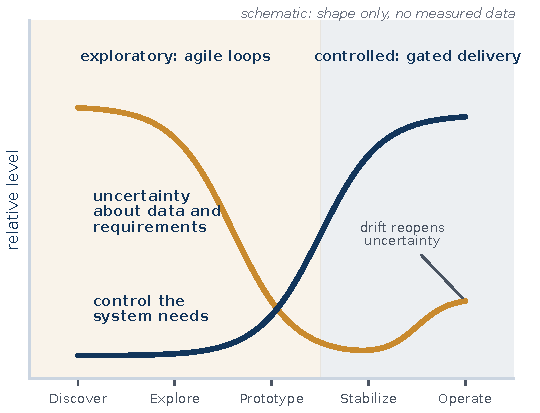
\includegraphics[height=5.0cm,keepaspectratio]{images/class23_uncertainty_vs_control.pdf}
\column{0.48\textwidth}
\begin{tikzpicture}
\badge{0.05}{-0.5}{coursegold}{compass}
\node[anchor=west, text width=5.5cm, align=left, font=\footnotesize] at (0.55,-0.5) {\textbf{Early phases are exploratory:} data quality, labels, and metrics are uncertain.};
\badge{0.05}{-1.85}{courseblue}{shield-alt}
\node[anchor=west, text width=5.5cm, align=left, font=\footnotesize] at (0.55,-1.85) {\textbf{Later phases need discipline:} deployment, interfaces, testing, and compliance.};
\badge{0.05}{-3.15}{coursered}{balance-scale}
\node[anchor=west, text width=5.5cm, align=left, font=\footnotesize] at (0.55,-3.15) {Regulated contexts cannot rely on verbal agreements or informal notebooks.};
\node[tileblue, anchor=north west, minimum width=6.2cm, text width=5.8cm, align=left, font=\scriptsize] at (0,-4.0) {\textbf{\color{courseblue}Example.} An industrial monitoring system may use agile prototyping for the predictor, then a more controlled process for deployment in the plant network.};
\end{tikzpicture}
\end{columns}
\coursefooter
\end{cframe}

\begin{cframe}{CRISP-DM: a process model made for data work}{\cterm{CRISP-DM}{Cross-Industry Standard Process for Data Mining: six phases for data projects.}\cterm{Business objective}{the outcome the organization wants, stated before any modeling.}}
\centering
\begin{tikzpicture}
\coordinate (C) at (3.2,-2.6);
\tikzset{ph/.style={tileblue, minimum width=2.0cm, minimum height=0.75cm, text width=1.8cm, font=\scriptsize\bfseries}}
\node[ph] (p1) at ($(C)+(0,2.0)$) {Business understanding};
\node[ph] (p2) at ($(C)+(2.1,1.0)$) {Data understanding};
\node[ph] (p3) at ($(C)+(2.1,-1.0)$) {Data preparation};
\node[ph] (p4) at ($(C)+(0,-2.0)$) {Modeling};
\node[ph] (p5) at ($(C)+(-2.1,-1.0)$) {Evaluation};
\node[ph, fill=coursegold!14, draw=coursegold] (p6) at ($(C)+(-2.1,1.0)$) {Deployment};
\node[circle, fill=courseice, draw=courseblue!40, minimum size=1.1cm, text=courseblue, font=\large] at (C) {\faIcon{database}};
\draw[arrow] (p1.east) -| (p2.north);
\draw[arrow] (p2.south) -- (p3.north);
\draw[arrow] (p3.south) |- (p4.east);
\draw[arrow] (p4.west) -| (p5.south);
\draw[arrow] (p5.north) -- (p6.south);
\draw[arrowgold] (p6.north) |- (p1.west);
\badge{7.0}{-0.55}{courseblue}{sync-alt}
\node[anchor=west, text width=5.9cm, align=left, font=\footnotesize] at (7.5,-0.55) {\textbf{Iteration is built in:} the phase sequence is not strict, and moving back and forth is expected.};
\badge{7.0}{-2.0}{coursegreen}{bullseye}
\node[anchor=west, text width=5.9cm, align=left, font=\footnotesize] at (7.5,-2.0) {\textbf{Evaluation} checks the results against the business objective, not only against a metric.};
\badge{7.0}{-3.5}{coursegold}{rocket}
\node[anchor=west, text width=5.9cm, align=left, font=\footnotesize] at (7.5,-3.5) {The last phase \textbf{plans monitoring and maintenance}; running models in production is the subject of MLOps (Class 26).};
\node[note, anchor=north west, text width=6.4cm] at (6.8,-4.75) {CRISP-DM 1.0 dates from 2000 and was written for data mining projects.};
\end{tikzpicture}
\coursefooter
\end{cframe}

\begin{cframe}{A hybrid lifecycle with gates}{\cterm{Gate}{a checkpoint where evidence decides whether work may move to the next stage.}\cterm{Exit criteria}{the conditions that must hold to pass a gate.}\cterm{Handoff rule}{who passes what to whom, and with what evidence.}}
\centering
\begin{tikzpicture}
\tikzset{st/.style={tileblue, minimum width=2.1cm, minimum height=0.8cm, text width=1.9cm, font=\scriptsize\bfseries}}
\tikzset{gt/.style={diamond, fill=coursered, text=white, font=\tiny\bfseries, inner sep=0.5pt, minimum size=0.6cm}}
\node[st, fill=coursegold!14, draw=coursegold] (a) at (1.05,0) {Discover problem};
\node[st, fill=coursegold!14, draw=coursegold] (b) at (3.5,0) {Explore data};
\node[st, fill=coursegold!14, draw=coursegold] (c) at (5.95,0) {Prototype model};
\node[gt] (g1) at (7.5,0) {1};
\node[st] (d) at (9.05,0) {Stabilize service};
\node[gt] (g2) at (10.6,0) {2};
\node[st] (e) at (12.15,0) {Operate and monitor};
\foreach \p/\q in {a/b, b/c, c/g1, g1/d, d/g2, g2/e} {\draw[arrow] (\p) -- (\q);}
\draw[arrowgold, rounded corners=6pt] (e.north) -- ++(0,0.7) -| (c.north);
\node[fill=white, font=\scriptsize\itshape, text=coursegray, inner sep=2pt] at (9.05,1.1) {feedback and change};
\fill[coursegold!40, rounded corners=1pt] (0,-0.62) rectangle (7.0,-0.74);
\node[font=\tiny\bfseries, text=coursegold!65!black, anchor=north west] at (0,-0.76) {EXPLORATORY: AGILE LOOPS};
\fill[courseblue!35, rounded corners=1pt] (8.0,-0.62) rectangle (13.2,-0.74);
\node[font=\tiny\bfseries, text=courseblue, anchor=north west] at (8.0,-0.76) {CONTROLLED: GATED DELIVERY};
\node[tilered, anchor=north west, minimum width=6.6cm, minimum height=1.55cm, text width=6.3cm, align=left, font=\footnotesize] at (0,-1.5) {{\bfseries\color{coursered}Gate 1: prototype to stabilize.} Example exit criteria: stakeholders accept a metric and a data source, and the requirements are testable.};
\node[tilered, anchor=north west, minimum width=6.6cm, minimum height=1.55cm, text width=6.3cm, align=left, font=\footnotesize] at (6.8,-1.5) {{\bfseries\color{coursered}Gate 2: stabilize to operate.} Example exit criteria: tests pass, the interface contract is stable, validation evidence is logged, and a fallback is defined.};
\keyidea{-3.35}{Match control to uncertainty: loops where the team is still learning, gates where a mistake becomes expensive.}
\end{tikzpicture}
\coursefooter
\end{cframe}

\begin{cframe}{Where do our projects sit?}{\cterm{Criticality}{how much harm a failure can cause.}\cterm{Release cadence}{how often new versions go live.}}
\begin{columns}[T]
\column{0.46\textwidth}
\centering
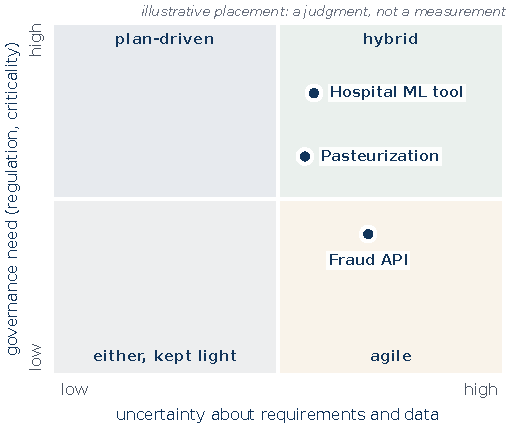
\includegraphics[height=5.0cm,keepaspectratio]{images/class23_process_positioning.pdf}
\column{0.52\textwidth}
\begin{tikzpicture}
\foreach \y/\ico/\name/\txt in {0/credit-card/Fraud API project/{Agile for feature and threshold iteration; structured release gates; monitoring after deployment.}, -1.85/thermometer-half/Pasteurization case/{Exploratory modeling can be agile; deployment gets stronger validation and change control.}, -3.7/hospital/Hospital ML support tool/{Stronger requirement control; formal validation and logging; slower but safer release cadence.}} {
  \node[tileblue, anchor=north west, minimum width=6.5cm, minimum height=1.7cm] at (0,\y) {};
  \badge{0.6}{\y-0.85}{courseblue}{\ico}
  \node[anchor=west, text width=4.9cm, align=left, font=\footnotesize\bfseries, text=courseblue] at (1.15,\y-0.33) {\name};
  \node[anchor=north west, text width=4.9cm, align=left, font=\scriptsize] at (1.1,\y-0.58) {\txt};
}
\end{tikzpicture}
\end{columns}
\coursefooter
\end{cframe}

\begin{cframe}{How to choose a process model}{\cterm{Boehm and Turner}{they rate a project on five factors to place it between agile and plan-driven.}}
\centering
\begin{tikzpicture}
\fill[coursegold!12] (6.0,-4.1) rectangle (13.7,0.55);
\node[anchor=west, font=\scriptsize\bfseries, text=coursegray] at (0,0.3) {QUESTION};
\node[anchor=west, font=\scriptsize\bfseries, text=coursegold!65!black] at (6.2,0.3) {PROCESS IMPLICATION};
\foreach \y/\ico/\q/\imp in {-0.45/anchor/Are requirements stable?/{More stability supports plan-driven structure.}, -1.25/database/Is data quality uncertain?/{More uncertainty favors iterative exploration.}, -2.05/balance-scale/Is the system regulated?/{More regulation requires stronger documentation and approval.}, -2.85/rocket/Are releases frequent?/{Frequent change favors incremental delivery and automation.}, -3.65/chart-line/Will the model evolve in production?/{Evolution demands monitoring and change governance.}} {
  \node[circle, fill=courseblue, text=white, minimum size=0.6cm, inner sep=0, font=\footnotesize] at (0.35,\y) {\faIcon{\ico}};
  \node[anchor=west, text width=5.0cm, align=left, font=\footnotesize\bfseries, text=courseblue] at (0.8,\y) {\q};
  \node[anchor=west, text width=7.3cm, align=left, font=\footnotesize] at (6.2,\y) {\imp};
  \draw[courseice!70!courseblue, line width=0.5pt] (0,\y-0.42) -- (13.7,\y-0.42);
}
\keyidea{-4.4}{These questions are an ML version of Boehm and Turner's five factors: size, criticality, dynamism, personnel, and culture. Rate your project on each before choosing.}
\end{tikzpicture}
\coursefooter
\end{cframe}

\begin{cframe}{Project checklist: what to defend in your presentation}{\cterm{Artifact}{anything the team produces that keeps others aligned: a document, a test, a dashboard.}}
\centering
\begin{tikzpicture}
\foreach \x/\y/\n/\ico/\q in {0/0/1/route/{Why did you choose this process?}, 6.8/0/2/sync-alt/{Where may the requirements still change?}, 0/-1.7/3/file-alt/{Which artifacts keep the team aligned?}, 6.8/-1.7/4/flag-checkered/{When do you move from experimentation to controlled delivery?}} {
  \node[tileblue, anchor=north west, minimum width=6.6cm, minimum height=1.5cm] at (\x,\y) {};
  \node[circle, fill=coursegold, text=white, font=\bfseries, minimum size=0.55cm, inner sep=0] at (\x+0.4,\y-0.4) {\n};
  \badge{\x+1.2}{\y-0.75}{courseblue}{\ico}
  \node[anchor=west, text width=4.6cm, align=left, font=\normalsize] at (\x+1.8,\y-0.75) {\q};
}
\keyidea{-3.5}{Be ready to defend each answer with an artifact from your project, not only with an argument.}
\end{tikzpicture}
\coursefooter
\end{cframe}

% ------------------------------------------------------------------ closing
\section{Wrap-up}\gdef\currentsectionname{Wrap-up}
\begin{frame}{From this class to the next}
\centering
\begin{tikzpicture}
\foreach \i/\lab/\bg/\fg in {1/SE and ML/courseblue!22/courseblue, 2/Requirements/courseblue!22/courseblue, 3/Process/courseblue/white, 4/Design/courseice/coursegray, 5/Quality/courseice/coursegray, 6/Evolution/courseice/coursegray} {
  \node[rounded corners=3pt, minimum width=2.18cm, minimum height=0.6cm, font=\scriptsize\bfseries, fill=\bg, text=\fg] at ({1.1+(\i-1)*2.28},0) {\i\ \lab};
}
\node[font=\tiny\bfseries, text=courseblue] at (5.66,-0.52) {THIS CLASS AND CLASS 25};
\foreach \x/\sty/\ico/\ttl/\txt in {0/tileblue/lightbulb/What stays with us/{$\bullet$\ No process is best everywhere; fit depends on uncertainty and governance.\\[3pt]$\bullet$\ ML needs iterative discovery without losing engineering control.}, 4.55/tileblue/project-diagram/Use it in your project/{$\bullet$\ Justify whether your work needs more loops, more structure, or a hybrid.\\[3pt]$\bullet$\ Define your gates and your definition of done.}, 9.1/tilegold/arrow-right/Next: Class 25/{\textbf{Agile Toolkit.}\\[3pt]Backlogs, stories, boards, ceremonies, and feedback loops. Class 24 is a guest session (YesAlps).}} {
  \node[\sty, anchor=north west, minimum width=4.3cm, minimum height=3.8cm] at (\x,-0.95) {};
  \badge{\x+0.65}{-1.6}{courseblue}{\ico}
  \node[anchor=west, text width=3.0cm, align=left, font=\small\bfseries, text=courseblue] at (\x+1.2,-1.6) {\ttl};
  \node[anchor=north west, text width=3.9cm, align=left, font=\scriptsize] at (\x+0.2,-2.25) {\txt};
}
\node[tilegold, fill=white, anchor=north west, minimum width=13.4cm, minimum height=0.95cm, text width=12.6cm, align=left, font=\footnotesize] at (0,-5.0) {{\bfseries\goldink\faIcon{route}\ Course thread.} After choosing a development posture, we turn it into everyday coordination practices a team can actually run.};
\end{tikzpicture}
\coursefooter
\end{frame}

% ------------------------------------------------------------------ references
\begin{frame}{References}
\centering
\begin{tikzpicture}
\refrow{0}{1.6}{book}{Books and guides}{Sommerville, I. \href{https://www.pearson.com/en-us/subject-catalog/p/software-engineering/P200000003144/9780137035151}{\emph{Software Engineering}}, Pearson.\\[2pt]Boehm, B. and Turner, R. (2003). \href{https://www.informit.com/store/balancing-agility-and-discipline-a-guide-for-the-perplexed-9780132651806}{\emph{Balancing Agility and Discipline: A Guide for the Perplexed}}.\\[2pt]Schwaber, K. and Sutherland, J. \href{https://scrumguides.org/}{The Scrum Guide}. \ \href{https://agilemanifesto.org/}{Agile Manifesto}.}
\refrow{-1.6}{1.95}{history}{History}{Royce, W. W. (1970). Managing the Development of Large Software Systems. \emph{Proc. IEEE WESCON}.\\[2pt]Takeuchi, H. and Nonaka, I. (1986). \href{https://www.scrum.org/resources/new-new-product-development-game}{The New New Product Development Game}. \emph{Harvard Business Review}.\\[2pt]Fowler, M. \href{https://martinfowler.com/articles/newMethodology.html}{The New Methodology}.}
\refrow{-3.55}{2.3}{robot}{Data and ML process}{Chapman, P. et al. (2000). \emph{CRISP-DM 1.0: Step-by-step data mining guide}.\\[2pt]Sculley, D. et al. (2015). \href{https://proceedings.neurips.cc/paper/2015/file/86df7dcfd896fcaf2674f757a2463eba-Paper.pdf}{Hidden Technical Debt in Machine Learning Systems}. NeurIPS.\\[2pt]Paleyes, A. et al. (2022). \href{https://arxiv.org/abs/2011.09926}{Challenges in Deploying Machine Learning: a Survey of Case Studies}. \emph{ACM Computing Surveys}.}
\end{tikzpicture}
\coursefooter
\end{frame}

\end{document}
